\section{Программирование интерфейса}
\subsection{Выбор среды разработки}

Первоначально интерфейс для работы с дельта-роботом предполагалось написать на основе Qt5 в среде разработки QtCreator. У меня были первоначальные наработки, связанные с предыдущим проектом фрезерного станка на Arduino. Планировалось использовать уже написанные ранее функции передачи данных через последовательный порт, для управления платой микроконтроллера. Тем не менее из-за некоторых проблем, связанных с регистрацией лицензии пробной версии QtCreator и внезапной невозможности сборки старого проекта (необходимо соблюдать версии IDE, компилятора и библиотек). Было принято решение полностью отказаться от Qt и использовать для написания интерфейса другую технологию.

В конечном итоге программа была написано с нуля на Python с применением библиотеки создания простых интерфейсов PySimpleGui. Данная библиотека идеально подходит для создания простых интерфейсов программ, без использования сторонних сред разработки. Существуют другие подобные аналоги, в частности Tkinter, который позволяет реализовать все стандартные виджеты, которые используются в интерфейсах программ:  кнопки, текстовые поля для ввода, надписи, скроллеры, списки, радиокнопки, флажки и другие. Но вариант PySimpleGui показался более интуитивно понятным. Не смотря на то, что у обоих вариантов есть свои "поваренные книги" с различными готовыми примерами стандартных окон, которые необходимо просто адаптировать под собственные нужды. Радует простота создания графического интерфейса, в предалах одного рабочего скрипта достаточно объявить библиотеку и в дальнейшем можно генерировать окна приложения обычными вызывами функций таким образом, каким это требуется. Простой интерфейс подразумевает, что у вас нет каталогизированного проекта, состоящего из различных по функционалу файлов. Есть только скрипт с необходимостью в определенный момент создать окно с несколькими стандартными виджетами, что реализуется несколькими строками кода.  

Хорошей особенностью PySimpleGui является наличие легко настраиваемых тем. Во-первых, существует несколько десятков стандартных тем, которые можно оценить, создав тестовый скрипт и прописав команду sg.theme\_previewer(). После запуска будут сгенерированны тестовые окна со всеми стандартными темами. В итоге, не нужно поочередно менять своему проекту все возможные варианты тем, а можно сразу подобрать самую привлекательную. В моем случае - DarkAmber. Подобный простейший функционал попросту отсутсвует в Qt Designer, так как подразумевается, что в коммерческом проекте дизайн будет профессиональным, разработанным с нуля и будет представлять некоторую стоимость с точки зрения авторского права. Но для решения простых, прикладных задач данный подход чрезвычайно трудоемок.

\subsection{Интерфейс программы}

Основная цель интерфейса программы - это удобная визуализация в одном месте всех переменных, которые используются внутри скрипта и обратная связь с пользователем. Для обратной связи служит многостроковое поле для текста, в котором выводятся сообщения о выполненных действиях скрипта. Я старался делать как можно больше сообщений, в самых критических местах, чтобы иметь возможность видеть на каких этапах произошел сбой. К сожалению, мне не удалось сделать вывод об ошибке о несуществующем последовательном порте, так как подобная проверка приводит к вылету программы с ошибкой о несуществующем порте. Вообще достаточно сложно программировать последовательный порт, из-за самых разных возникающих проблем. Для простоты, я решил предположить, что пользователь знает имя последовательного порта, по которому подключен микроконтроллер и в данном месте не делать проверок.

\begin{figure}[h!]
\centering
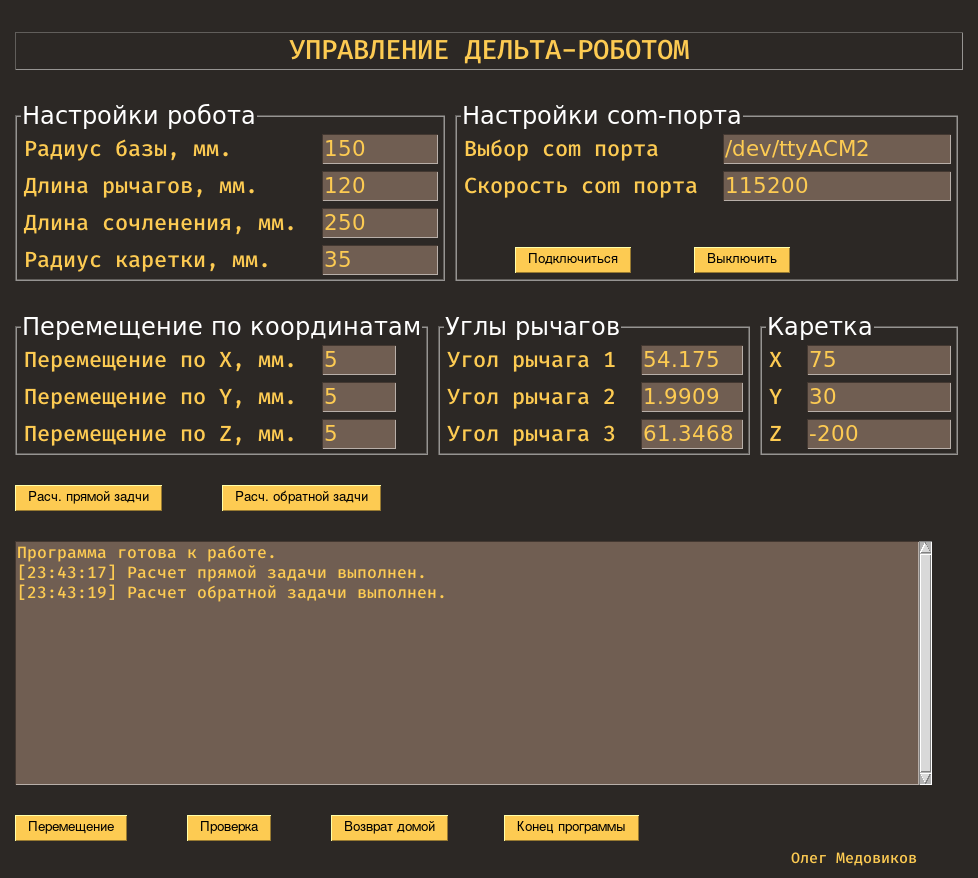
\includegraphics[width=0.8\linewidth]{./image/gui}
\caption{Интерфейс программы управления дельта-роботом}
\end{figure}

Интерфейс состоит из нескольких блоков переменных, которые разделены логически и визуально, как и в графическом виде, так и внутри скрипта, для простоты работы и пользователя и программиста. 


\begin{lstlisting}[style=python,caption=Использование PySimpleGui]

import PySimpleGUI as sg

sg.theme('DarkAmber')   # Цветовая схема

layout = [ # Наполнение окна: текстовое поле и кнопка
[sg.Text('Oleg',font=("Fira Code",16)), sg.Button('Example')],
            ]

while True:  # Цикл вызова окна
    event, values = window.read()

    if event == 'Example':   # Действие при нажатии 
        primaiaZadacha()


window.close()
\end{lstlisting}

Наполнение окна виджетами записывается в виде двойного массива $layout = [ [witget1], [witget2]]$. Для создания блоков, формируются особые виджеты фреймы, которые можно расписывать аналогично, в виде двойного массива виджетов.В минус данной библиотеки можно записать то, что по умолчанию используется не квадратный шрифт, возможно, подхватывается какой-то из системных шрифтов. Не квадратный шрифт подразумевает, что разные буквы могут иметь разную ширину в пикселях. Так как расположение полей ввода регулируется с помощью текстового блока слева, с таким шрифтом их невозможно расположить ровно, если надписи разные. Поэтому я использовал шрифт Fira Code.

\subsection{Поля с переменными движения}

При расчете параметров движения используются поля, где указаны главные параметры дельта-робота в миллиметрах. Все параметры интерактивны и функции расчета движения каждый раз берут именно те значения, которые в данный момент отображены в полях. По умолчанию в полях отображаются значения робота, воплощенного в експериментальной модели.


Поля <<Перемещение по координатам>> необходимы для ввода значений, на которое требуется изменить коодинаты каретки робота. Поля используются только для работы кнопки <<Перемещение>>. Логика программы подразумевает, что пользователь апперирует координатами, а микроконтроллер углами рычагов. Поэтому, когда пользователь заносит требуемое изменение координат в миллиметрах, программа решает обратную задачу управления и получает углы, соответсвующие этим координатам. Углы нормализуются, переводятся в шаги шаговых двигателей и отправляются в  Arduino, которая заставляет двигатели совершить нужное количество шагов.

Поля <<Углы рычагов>> и <<Каретка>> отображают значение углов рычагов в градусах и координаты каретки в миллиметрах. Данные поля используются функциями расчета прямой и обратной задачи, которые берут из них значения и обновляют при завершении расчетов.

\begin{lstlisting}[style=python,caption=Получение и обновление значения виджета]
frame_delta = [
    [sg.Text('Number',font=("Fira Code",16)),
    sg.InputText('150',size=(8,1),font='any 16',key='value')],
                ]

N  = float(values['value'])

N = N + S

 window['value'].update(str(round(N,2)))
\end{lstlisting}

Получить значение из виджета можно при условии, что указан ключ - показатель данного значения. Необходимо помнить, что значение внутри виджета всегда будет иметь формат строки. Поэтому для проведения математических операций необходимо сменить формат переменной, например, на float. Я решил не использовать целочисленные форматы, для увеличения точности. После проведения математических операций, для обновления значения в виджете, необходимо обратно вернуть формат строки string. Дополнительно в примере происходит округление до двух знаков после запятой.

Ключ можно использовать для всех необходимых виджетов, не обязательно использовать именно InputText.

\subsection{Настройка com-порта.}
Блок отличается наличием конопок на открытие и закрытие канала по последовательному порту. Из-за нехватки времени не реализованна функция сканирования существующих или доступных портов, выбор происходит путем написания имени порта в текстовое поле. К сожалению, в данный момент если прописать в поле несуществующий порт, то при попытке подключения программа аварийно завершается с ошибкой о несуществующем порте. Требует доработки.

Использование паралельного порта происходит при помощи библиотеки Pyserial.

\begin{lstlisting}[style=python,caption=Пример использования Pyserial]
import serial

if event == 'Connect':
    ser = serial.Serial(
            port=values['serial'],
            baudrate=values['serial_v'],
            parity=serial.PARITY_ODD,
            stopbits=serial.STOPBITS_TWO,
            bytesize=serial.SEVENBITS
            )
    ser.isOpen()

    window['pole'].update(time + 'Connection'
        + values['serial'] + ' successfull.',append=True)

if event == 'Close':
    ser.close()
    window['pole'].update(time + 'Close connection'
        + values['serial']+'.',append=True)

\end{lstlisting}

Используемые переменные: имя порта, которое меняется в процессе эксплуатации. И скорость передачи данных по последовательному порту, которое я выбрал равным 115200 бит в секунду. Скорость может быть ограничена длинной кабеля или шумами наводки, но в моей ситуации провод короткий и шумы отсутвуют. Скорость передачи обязательно должна согласоваться с настройками в прошивке Arduino, поэтому данный параметр нельзя менять просто так.

\paragraph{Передача символов}

Команды на выполнение определенных действий задаются символами в кодировке UTF-8. Данная программа отправляет несколько символов микроконтроллеру:

T - простая проверка наличия связи с микроконтроллером, который должен вернуть символ Y. Если это происходит, то проверка пройдена, иначе появляется сообщение об ошибке.

H - команда отправить каретку в исходную позицию. Для того, чтобы совершить данное действие, микроконтроллеру не нужно знать положение каретки и количество необходимых шагов. Функция будет выполняться пока, не сработают все концевики и плата не отправит потверждение о выполнении Y.

C - команда о смене координат. После получения данной буквы, контроллеру необходимо получить углы рычагов, выраженные через количество шагов двигателей. После чего контроллер находит разность между полученными углами и хранящимися в памяти и запускает функцию движения на необходимую дельту. При этом координата каретки обновляется в памяти контроллера. После выполнения функции движения, происходит отправка потверждающей буквы О.

\begin{lstlisting}[style=python,caption=Отправка символа через параллельный порт]

ser.flush()
ser.write(str.encode('T'))
t = str(ser.read(2).decode("utf-8"))
if t == 'TY':
    window['pole'].update(time + 'connection to Arduino' + 
         'was successful.',append=True)
else:
    window['pole'].update(time + 'connection to Arduino' + 
         'with an error.',append=True)

\end{lstlisting}

Рассмотрим процесс передачи смвола на примере совершения проверки. Для начала необходимо очистить буфер порта, чтоб избаться от возможных ошибок, связанных с наличием в буфере остаточных данных. Это делается командой flush(). После происходит непоредственная запись в порт команды и чтение буфера. Конечно, она представляет собой 8 бит, нулей и единиц, но так как человеку удобнее оперировать именно буквами, в команде указывается в какой именно кодировке мы хотим увидеть конечный результат. Чтение происходит двух символов, так как если читать один символ, то скрипт прочитает тот же символ, который только что отправил. Необходимо прочитать именно два символа, чтобы сформировать комбинацию команда-ответ. Если переменная t приняла значение TY, это значит, что команда и ответ были отправлены. Если на ответ микроконтроллеру требуется время (например, необходимо выполнить перемещение каретки), то функция Read будет ожидать ответа несколько секунд, чего вполне достаточно при стандартной работе робота.  

\subsection{Прямая и обратная задача}

Функция решения прямой задачи управления дельта роботом реализована аналогично, как и в Zencad, кроме необходимости вытаскивать значения из полей ввода окна программы. И небольшого нюанса с переводом значений градусов в радианы. Для чего пришлось добавить небольшую функцию deg(), которая есть в ZenCad по умолчанию. 

\begin{lstlisting}[style=python,caption=Функция перевода градусов в радианы]
def deg(k):
    return k * math.pi / 180
\end{lstlisting}


Функция решения обратной задачи реализованна, как двойная функция. Так по алгоритму необходимо трижды выполнить аналогичные действия, внутри функции объявлена другая функция, к которой первая обращается при необходимости. Основная функция служит только для получения начальных условий для второй и вывода конечных результатов. Координаты X,Y,Z трижды отправляются во вторую функцию, которая работает для всех рычагов, как для первого рычага, только потому, что происходит вращение координат. Каждый из рычагов по очереди становится первым.

\begin{lstlisting}[style=python,caption=Основная функция обратной задачи]
def obratnaiZadacha():

    X     = float(values['X'])
    Y     = float(values['Y'])
    Z     = float(values['Z'])

    teta1 = calcTeta1(X,Y,Z)

    X2 = X*math.cos(deg(120)) + Y*math.sin(deg(120))
    Y2 = Y*math.cos(deg(120)) - X*math.sin(deg(120))
    teta2 = calcTeta1(X2,Y2,Z)

    X3 = X*math.cos(deg(-120)) + Y*math.sin(deg(-120))
    Y3 = Y*math.cos(deg(-120)) - X*math.sin(deg(-120))
    teta3 = calcTeta1(X3,Y3,Z)

    window['teta1'].update(str(round(teta1,4)))
    window['teta2'].update(str(round(teta2,4)))
    window['teta3'].update(str(round(teta3,4)))
    window['pole'].update(time + 'Calculation completed.'
                            ,append=True)

\end{lstlisting}

Решение основано на нахождении корней квадратного уравнения, приведенного в первой главе. Здесь находятся координаты "локтя" именно первого рычага, потому что он расположен таким образом, что его координата по Х ($J_{x}$) всегда равна нулю. Поэтому решается система из двух неизвесных, а не из трех. В оригинальном коде, существовала проверка, что Y координата локтя больше Y координаты крепелнеия каретки ($J_{y} > y_{1}$). В данной конструкции робота подобная ситуация невозможна, так как максимальный угол поворота рычага ограничен $90^{\circ}$, но проверка оставлена. Дело в том, что при дальнешем вращении рычагов, каретка вместо движения вниз пойдет вверх. В итоге для одних и тех же координат в самой нижней рабочей области получится два решения. Чтобы это избежать, необходим запрет на поворот ондновременно трех рычагов более чем на $90^{\circ}$. Поворот двух рычагов более чем на $90^{\circ}$ позволит увеличить максимальное перемещение каретки в сторону от значения радиуса базы на еще 15-20\%.      

\begin{lstlisting}[style=python,caption=Вспомогательная функция обратной задачи]
    def calcTeta1(X,Y,Z):
        rad   = float(values['f'])
        e     = float(values['e'])
        Rf    = float(values['rf'])
        Re    = float(values['re'])

        y1 = -rad
        Y = Y - e

        a = (X**2 + Y**2 + Z**2 + Rf**2 - Re**2 - y1**2)/(2*Z)
        b = (y1 - Y) / Z

        d = -( (a + b*y1)**2 ) + (b**2 + 1)*Rf**2
        if d < 0 :
            window['pole'].update(time + 'Wrong characteristics'
                + ' of the robot, no roots.',append=True)
            return 0
        else:
            Jy = (y1 - a*b - math.sqrt(d)) / (b**2 + 1)
            Jz = a + b*Jy
            if Jy > y1 :
                k = 180
            else:
                k = 0
            return  180*math.atan(-Jz/(y1 - Jy)) /math.pi + k


\end{lstlisting}

Так как в программе реализованы обе задачи прямого и обратного решения, то очень легко проверить корректность работы обеих функций. Для этого достаточно запустить расчет прямой задачи и из углов рычагов получить координаты коретки. После запустить обратную задачу и получить из координат коретки углы рычагов. Если в процессе выполнения данных функций в любом порядке углы и координаты не меняются, то это с большой вероятностью гарантирует правильность расчетов. Расчтеты могут меняться из-за погрешности вызванной округлением, но в проверенных мной случаях, округления до второго знака после запятой вполне достаточно. 

Данными функциями также можно проверять возможность создания дельта-робота с определенными параметрами, так как в случае невозможности конструкции, функция предупредит об этом. 

\subsection{Работа кнопки <<Перемещение>>}

Перед отправкой команд микроконтроллеру необходимо получить необходимое количество шагов. Из полей координат берется текущее положение в пространстве. Для правильного выполнения алгоритма, программу необходимо начинать с возвращения каретки домой, то-есть в начальное положение. Это единственный способ актуализировать программные координаты с физическими координатами каретки. Из полей перемещения по координатам берется значение разности координат и считается конечное положение.

\begin{center}
    $X_{2} =  X_{1} + \Delta$
\end{center}

Конечное положение округляется до второго знака и возращается в поля текущего положения, чтобы можно было начать решать обратную задачу управления роботом.

\begin{lstlisting}[style=python,caption=Получение количества шагов]

if event == 'Movement':
    X  = float(values['X']) + float(values['dx'])
    Y  = float(values['Y']) + float(values['dy'])
    Z  = float(values['Z']) + float(values['dz'])

    window['X'].update(str(round(X,2)))
    window['Y'].update(str(round(Y,2)))
    window['Z'].update(str(round(Z,2)))

    obratnaiZadacha()

    k =  float(values['Ndvig']) * float(values['Kred'])/360

    teta1  = round(k*(float(values['teta1']) + 15))
    teta2  = round(k*(float(values['teta2']) + 15))
    teta3  = round(k*(float(values['teta3']) + 15))


\end{lstlisting}

После выполнения функции обратной задачи в полях углов появляются требуемые значения углов в градусах. Перевод в шаги происходит с помощью формулы количества шагов на весь диапазон вращения рычагов. В данном случае количество шагов необходимо разделить на количество градусов на диапозон, но это значение уже было в формуле, можно его сократить. К значению угла нужно прибавить минимальное значение угла, чтобы избежать отрицательных значений угла. Для избежания дробных значения шагов, происходит округление до целого. 

\begin{center}
    $N_{shagov} = \frac{\theta_{max} - \theta_{min} }{360^{\circ}}* N_{dvig} * K_{reductor} $\\
    \vspace{0.5cm}
    $\theta_{step} = \frac{N_{dvig} * K_{reductor}}{360^{\circ}}*(\theta^{\circ} + \theta^{\circ}_{min})$

\end{center}

После получения значений углов, выраженное в количестве шагов, необходимо дать микроконтроллеру команду на изменение координат. После чего он поочередно запросит значения переменных. Так как значения больше 255 и могут быть отрицательными, то они не укладываются в один байт информации, необходимо использовать переменную типа Integer, которая занимает 4 байта. Для передачи через параллельный порт переменной Int используется возможность Python создавать структурные пакеты. Буква i внутри функции struct.pack() обозначает тип переменной value, а именно Int. Данная функция раскладывает переменную Int на 4 байта, которые можно поочередно отправить в микроконтроллер.  

\begin{lstlisting}[style=python,caption=Преобразование Int в пакет]
import struct

def packIntegerAsULong(value):
    \\Packs a python 4 byte integer to an arduino
    return struct.pack('i', value)

\end{lstlisting}

Первым делом перед отправкой команды на микроконтроллер, происходит обязательная очистка буфера com-порта. После отправки символа C, микроконтроллер должен ответить запросом значения X. В данном случае, это не запрос координаты X, а запрос угла $\theta_{1}$. Так как работать приходится с одним символом, то удобно обозвать первый, второй и третий угол рычага буквами X, Y, и Z. 

Если скрипт читает в буфере два символа CX, то в поля программы выводится сообщения об изменении углов и их числовое значение в шагах. И происходит передача первого угла. Скрипт очищает буфер параллельного порта.

Если микроконтроллер принимает число, то отправляет символ Y. Если скрипт читает символ Y, то отправляет значение второго угла. Скрипт очищает буфер параллельного порта.

Если микроконтроллер второе число, то отправляет символ Z. Если скрипт читает символ Z, то отправляет значение третьего угла. Скрипт очищает буфер параллельного порта.

Когда микроконтроллер получает третье число, он находит разность с текущими значениями углов и запускает функцию движения на значение разности. Обновляет координаты. После выполнения движения, отправляет символ О.

Если скрипт получает символ О, то в поле программы выводится сообщение об успешном окончании движения.



\begin{lstlisting}[style=python,caption=Команда на перемещение каретки]
ser.flush()
ser.write(str.encode('C'))
c = str(ser.read(2).decode("utf-8"))
if c == 'CX':
    window['pole'].update(time + 'Change pozition'
        + str(X) + '  '+ str(Y) +'  '+ str(Z) ,append=True)

    ser.write(packIntegerAsULong(teta1))

ser.flush()
c = str(ser.read(1).decode("utf-8"))
if c == 'Y':
    ser.write(packIntegerAsULong(teta2))

ser.flush()
c = str(ser.read(1).decode("utf-8"))
if c == 'Z':
    ser.write(packIntegerAsULong(teta3))

ser.flush()
c = str(ser.read(1).decode("utf-8"))
if c == 'O':
    window['pole'].update(time + 'Carriage moved',append=True)

\end{lstlisting}

В данном скрипте не предусмотрена возможность ошибки при появлении неправильных символов или потере связи. Если микроконтроллеру нужно достаточное время на отправки символа, скрипт будет находится в ожидании, пока не появится какой-либо символ.

\subsection{Выводы}

Наличие подключения через параллельный порт является самым узким местом проекта. Изначально подразумевалось, что роботом управляет одноплатный компьютер, на котором запускается скрипт Python, который управляет микроконтроллером по средством отправки символов. Но это подключение работает очень сложно и неочевидно. Передача данных сильно осложнена, и нужно написать еще несколько функций, например такую, что  сообщает компьютеру о срабатывании концевиков. Очень спорная ситуация, что Arduino и компьютер считают текущие значения углов обособленно друг от друга. Было бы правильнее расчитывать текущие углы на компьютере и отправлять на Arduino только количество необоходимых  шагов, но это повышает вероятность ошибки, так как компьютер не знает физического положения каретки. Само наличие связи через параллельный порт требует скурпулезной отработки всех возможных ситуаций. В случае приема неправильных символов необходимо придумать алгоритмы отработки ошибки, чтобы ее невелировать и начать выполнение функции заново. Происходит нагромождение логики и изначально простые и стройные функции превращаются в логические лабиринты, которые можно было бы избежать, убрав параллельный порт из системы.

